\chapter{Sprint3: Déploiement de l'application sur le cluster.}
\newpage
\textbf{\huge Introduction} \\[1cm]

\textsf{\fontfamily{qtm}\selectfont\scalefont{1.3}
Après avoir déduit la configuration du pipline nous présentent la troisieme  sprint, nous commençons par l'objectif de sprint puis l'architecture globale ensuite nous détaillons le diagramme d'utilisation et séquence détaille, Finalement, nous allons exposer la partie réalisation}


\section{\LARGE Objectif du Sprint}
\textsf{\fontfamily{qtm}\selectfont\scalefont{1.3} l'objectif du déploiement de l'application sur un cluster est d'assurer une disponibilité élevée, une évolutivité, une tolérance aux pannes, une gestion efficace des ressources, une sécurité, une facilité de déploiement et une surveillance pour fournir une expérience utilisateur optimale dans un environnement de cluster.}


\section{\LARGE Architecture Détaillée}
\textsf{\fontfamily{qtm}\selectfont\scalefont{1.3}Dans cette partie nous allons présenter l'architecture détaillée correspond au sprint.}

\subsection{\Large Diagramme Cas d'utilisation Détaillée}
\textsf{\fontfamily{qtm}\selectfont\scalefont{1.3}Afin d'éliminer toute ambiguïté et de clarifier le cas d'utilisation, nous présentons le cas de façon détaillée.}

\begin{figure}[H]
    \begin{center}
    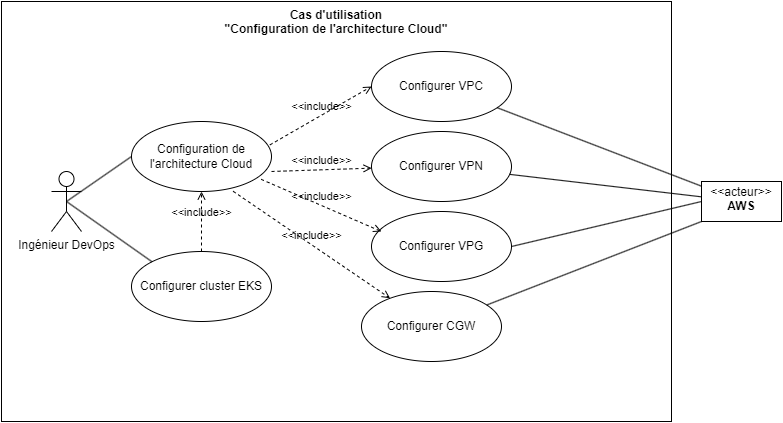
\includegraphics[height=10cm]{usecasedet.drawio.png}
    \end{center}
    \caption{cas d’utilisation"Déploiement de l'application sur
le cluster."}
    %\floatfoot{Source: (Citation command)}
    % avec le package "floatrow"
    \end{figure}

  \textsf{\fontfamily{qtm}\selectfont\scalefont{1.3}
    Pour expliquer  le diagramme de cas d’utilisation, nous représentons la description textuelle du principales fonctionnalités mentionnées ci-dessus : \\}
    \begin{center}
       \begin{table}[H]  
         \centering
         \resizebox{1.1\textwidth}{!}{%
         \begin{tabular}{|c|p{13cm}|}
          \hline
          Titre & Déploiement de l'application sur
le cluster.\\
          \hline
          Acteur & Ingénieur DevOps \\
          \hline
          Description & L'ingénieur DevOps gérait transférer l'application et ses composants dans un environnement de cluster, dans lequel elle peut être exécutée et gérée de façon efficace et évolutive .\\
          \hline
          Pré conditions & La configuration de cluster ainsi la configuration de l'application et la gestion des depandances . \\
          \hline
          Post conditions & l'application deploye sur cluster et bien fonctionne .  \\
          \hline 
          Scénario nominal &  l'application est déployée avec succès sur le cluster, fonctionne de manière stable et répond aux exigences spécifiées.\\
          \hline
          Scénario alternatif & problèmes lors de la configuration du cluster ou  problèmes de configuration de l'application , de réseau ou de ressources insuffisantes.  \\
          \hline
          \end{tabular}%
         }
       \caption{Description de cas d’utilisation}
       \end{table}
       \end{center}